%\documentclass[a4paper]{article}
%
%%% Language and font encodings
%\usepackage[english]{babel}
%\usepackage[utf8x]{inputenc}
%\usepackage[T1]{fontenc}
%\usepackage[noadjust]{cite}
%\usepackage{booktabs}
%\usepackage{subcaption}
%\renewcommand{\citedash}{--}  
%%% Sets page size and margins
%\usepackage[a4paper,top=3cm,bottom=2cm,left=3cm,right=3cm,marginparwidth=1.75cm]{geometry}
%
%%% Useful packages
%\usepackage{amsmath}
%\usepackage{url}
%\usepackage{graphicx}
%%\usepackage[colorinlistoftodos]{todonotes}
%\usepackage[colorlinks=true, allcolors=blue]{hyperref}
%
%\title{\textsc{Theia} DBD White Paper}
%%\author{T. Klosterman, V. Lozza, A. Mastbaum}
%
%\begin{document}
%\maketitle

%\section{Introduction}
The \textsc{Theia} search for neutrinoless double beta decay (NLDBD) aims for
sensitivity to the non-degenerate normal hierarchy parameter space
within the canonical framework of light Majorana neutrino exchange and
three-neutrino mixing, at the level of $m_{\beta\beta}\sim5$ meV.
This is achieved through the loading of a very large
mass of a NLDBD candidate isotope into an ultra-pure liquid scintillator
target, together with coincidence and topological particle identification
techniques.

\subsubsection{Detector Configuration}
\paragraph{Target Medium}
For the present studies, we consider a target that consists of pure LAB
liquid scintillator loaded with the NLDBD isotope. This volume is contained
within a nylon balloon, and the region of the detector outside is
filled with water-based liquid scintillator (WbLS) with no isotope loading.
With loading at 3\% by mass, a 25 ton (50 ton) experiment corresponds to a
6.4 m (8 m) radius containment balloon.

The mass of LAB is obtained using a density of 0.86 g/cm$^3$, the optics are
based on measurements by the SNO+ collaboration, and the backgrounds are based
on measurements by SNO+, Borexino, and KamLAND-Zen.

\paragraph{Isotope Loading}
We consider possible NLDBD searches using two candidate isotopes: Te and Xe.
In the case of Xe loading, xenon gas 89.5\% enriched in $^{136}$Xe is
dissolved directly into
the liquid scintillator, while Te loading is achieved via a novel
technique developed for the SNO+ experiment
and uses natural Te (34.1\% $^\mathrm{130}$Te).
The contamination associated with the materials used for Te loading are
considered in the background assessment.

Additional NLDBD isotopes may be considered as long as they can be loaded into
liquid scintillator. A staged approach is envisioned where an
NLDBD observation in one isotope can be confirmed by removing it and deploying
a second; the ability to switch isotopes is a key advantage of a liquid
scintillator detector.

\subsubsection{Backgrounds}
The main sources of background near the NLDBD energy region of interest
include:
\begin{description}
\item[Double Beta Decay] This irreducible background is due to the
$2\nu\beta\beta$ decays of $^{130}$Te or $^{136}$Xe. Due to the steeply-falling
spectrum, the number of events falling in the ROI depends strongly on the
energy resolution.
\item[Cosmogenic Production] These backgrounds are due to activation of nuclei
by muons (during data taking) or protons and neutrons (during material
production and handling at Earth's surface).
\item[Solar Neutrinos] The primary source is elastic scattering of $^{8}$B
solar neutrinos, though these events can potentially be reduced using the
direction relative to the Sun. Another potential background is due to
activation of the target material (Te or Xe) by the solar neutrinos,
mainly $^{7}$Be and $^{8}$B neutrinos; this background is also dependent
on the energy resolution.
\item[Internal Contamination] Decays from U- and Th-chain impurities
present in the scintillator mixture. Due to the large $Q$ value of the
candidate NLDBD isotopes, the two important backgrounds are due to
$^{214}$Bi ($Q=3.27$ MeV) and $^{208}$Tl ($Q=5$ MeV). The scintillator
purity can be improved by purification techniques to levels better than
$10^{-18}$, as demonstrated by the Borexino experiment \cite{bxo16}.
\item[External Sources] Decays from U and Th-chain impurities present
in the balloon material, the external water-based liquid scintillator, the
shielding water, and in the PMTs also contribute to the background. The
two most important isotopes are $^{214}$Bi and $^{208}$Tl, as they decay by
the emission of high energy ($E>2$ MeV) $\gamma$ rays that can travel long
distances. These events can be reduced using a fiducial volume cut, though the
balloon material remains the most important as it is closest to the target
volume.
\end{description}
A summary of all the expected background events is given in Table
\ref{tab::bckg}.

\begin{table}[t]
\centering
\begin{tabular}{lccc}
\toprule
                                            &                                              & \multicolumn{2}{c}{\bf Expected events/y}     \\
{\bf Source}                                & {\bf Target level}                           & $r = 6.4$ m           & $r = 8$ m             \\
\midrule
Balloon $^{10}$C                            &                                              & 250 -- 800            & 500 -- 1600           \\
$^{8}$B neutrinos                           &                                              & 1490                  & 2950                  \\
$^{130}$I (Te target)                       &                                              & 48 (9 from $^{8}$B)   & 93  (18 from $^{8}$B) \\
$^{136}$Cs (Xe target)                      &                                              & 24 (3 from $^{8}$B)   & 47 (6 from $^{8}$B)   \\
$^{136}$Cs ($^\mathrm{enr}$Xe target)       &                                              & 245 (35 from $^{8}$B) & 478 (68 from $^{8}$B) \\
2$\nu\beta\beta$ (Te target)                &                                              & 3.8$\times$10$^{7}$   & 7.4$\times$10$^{7}$   \\  
2$\nu\beta\beta$ (Xe target)                &                                              & 3.6$\times$10$^{6}$   & 7.0$\times$10$^{6}$   \\  
2$\nu\beta\beta$ ($^\mathrm{enr}$Xe target) &                                              & 3.6$\times$10$^{7}$   &  7.1$\times$10$^{7}$  \\  
Liquid scintillator                         & $^{214}$Bi: $10^{-17}$ g$_{U}$/g             & 3700                  & 7300                  \\
                                            & $^{208}$Tl: $10^{-17}$ g$_{Th}$/g            & 440                   & 870                   \\
Nylon Vessel                                & $^{214}$Bi: 1.1$<\times10^{-12}$ g$_{U}$/g   & 7.7$\times$10$^{4}$   & 1.2$\times$10$^{5}$   \\
                                            & $^{208}$Tl: 1.6$<\times10^{-12}$ g$_{Th}$/g  & 1.3$\times$10$^{4}$   & 2.1$\times$10$^{4}$   \\
PMTs                                        & $^{214}$Bi: $10^{-6}$ g$_{U}/$PMT            &                                               \\
                                            & $^{208}$Tl: $10^{-6}$ g$_{Th}/$PMT           &                                               \\
\bottomrule
\end{tabular}
\caption{Dominant background sources expected for the NLDBD search in
\textsc{Theia}. It is assumed that the Te or Xe isotopes are directly
loaded at a level of 3\% in the LAB+PPO scintillator cocktail, for a
total mass of 28.3 tonnes (6\,m radius) or 55\,tonnes (8\,m radius).}
\label{tab::bckg}
\end{table}

\paragraph{Cosmogenic Backgrounds}
The cosmogenically-induced background consists of nuclides produced by
activation of the target material by neutrons, protons, and muons during
production, handling, storage, and data-taking.

Long-lived, high $Q$ value nuclides can be produced by neutron and proton
activation mainly while the material is on the Earth's surface. The production
in Xe and Te has been investigated by several authors
\cite{mei09, baudis15, zhang16, norm05, bard97, wang15, lozza15}. Among
the most important nuclides are $^{60}$Co ($Q=2.8$ MeV, $T_{1/2}=5.27$ y) and
$^{110m}$Ag ($Q=3.1$ MeV, $T_{1/2}=250$ d). Mitigation of these background
sources requires minimal exposure at sea level, a deep underground cool-down
period, and chemical purification processes \cite{snop16}.

Neutron activation can also happen deep underground, while the experiment is
running. Neutrons originate from the radioactivity and from muon-induced
reactions in the rock. A water shield will provide a mitigation, as the
majority of the neutrons will thermalize and stop before reaching the target
material.

For the purpose of this paper, it is assumed that the material will have a
minimum exposure time at sea level and will be stored underground long
enough to allow all the potential cosmogenic-induced nuclides produced during
the surface exposure to decay.\\

A different source of cosmogenic background is the muon activation of the
material during the data-taking period. In particular a potential background
is the production of $^{10}$C ($Q=3.65$ MeV, $T_{1/2}=19.3$ s) by muon
interaction with the carbon atoms of the liquid scintillator. The interaction
is accompanied by the emission of two neutrons. $^{10}$C decays via the
emission of a positron of 1.87\,MeV end-point energy, followed by the
emission of a $\gamma$ of 0.72\,MeV total energy. A mitigation strategy for
this background source consists of a three-fold coincidence technique as
developed by Borexino and KamLAND \cite{galb05, gando16}, making use of the
muon trajectory, the 2.2\,MeV $\gamma$ emitted by the neutron capture, and
the $^{10}$C decay. Additionally, the $\gamma$ may travel away from the
positron stopping point several tens of centimeters. This event topology is
different from the neutrinoless double-beta decay, in which the energy
deposition is localized.

The event rate of muon induced $^{10}$C decays can be estimated following
Reference \cite{hagn00}. The muon flux expected at the Homestake 4850 level
(4300 mwe) is $4.2\times10^{-9}$ cm$^{-2}$ s$^{-1}$, while the calculated
average muon energy at the same depth is 293\,GeV \cite{mei06}. The
LAB+PPO mixture has a $^{12}$C density of $4.4\times 10^{31}$ atoms/kt.
The following formula can be used to scale the density from the one measured
in Borexino and KamLAND:
\begin{equation}
R_{i} = R_{data} \times 
{\left( \frac{\langle E_{\mu} \rangle}
             {\langle E_{\mu, data} \rangle} \right) }^{\alpha_{sim}} \times
\frac{\Phi_{\mu}}{\Phi_{\mu, data}} \times
\frac{n_{12C}}{n_{12C, data}}
\end{equation}
where $\alpha_{sim}$ has been obtained from FLUKA/Geant4 simulation and is
equal to 0.7621 for $^{10}$C \cite{zbiri10}. This results in about 300
events/kt/yr. Using Equation 10 in Reference \cite{hagn00} results in about
800 events/kt/yr. For this source of background a reduction of 92.5\% is assumed based on what reached by Borexino \cite{bxo2013}

\paragraph{Solar Neutrino Induced Background}
$^{8}$B solar neutrino elastic scattering in the target material results in
a background that is approximately flat across the NLDBD energy region of
interest. The spectrum can be normalized using the total $^{8}$B flux and
best fit solar mixing parameters, as in Reference \cite{SNO_3ph}. The expected
rate is about 1200 events/yr/kt of target material.\\

Another source of background are the nuclides produced by charged current
interaction of solar neutrinos with Te or Xe, in particular $^{130}$Te and
$^{136}$Xe. A detailed study of the expected interaction rate is given in
References \cite{eijiri14, eijiri17}. 

For $^{130}$Te (34.08\% natural abundance) a total of 33.7 SNU are expected,
of which 6.1 SNU due to $^{8}$B neutrinos and 20.9 SNU due to $^{7}$Be
neutrinos. The daughter isotope is $^{130}$I in the 1$^{+}$ excited state.
The excited states decay quickly to the first excited level, which decays with
$T_{1/2}=8.84$ min to the ground state via internal transition (branching
ratio 84\%, $E_\gamma=40$ keV), or directly beta decays to $^{130}$Xe with a
$Q$ value of 2.99\,MeV (BR = 16\%). The ground state beta decays with a
$Q$ calue of 2.95\,MeV and a $T_{1/2}=12.4$\,h. Due to the long half life a
tagging technique based on a delayed coincidence might have a small efficiency.

For $^{136}$Xe (8.8573\% natural abundance) a total of 68.8 SNU are expected,
of which 9.8 SNU due to $^{8}$B neutrinos and 46 SNU due to $^{7}$Be neutrinos.
The resulting isotope is $^{136}$Cs in the 1$^{+}$ excited states. The
excited states decay quickly to the ground state, which decays with
$T_{1/2}=13.16$\,d via beta decay (branching ratio = 100\%) with a $Q$ value
of 2.55\,MeV. Again in this case, a tagging technique
based on a delayed coincidence will have only a small effect on removing this
source of background due to the long half life.

The expected rate of events is given in Table \ref{tab::bckg}.

\paragraph{Double Beta Decay Backgrounds}

The number of 2$\nu\beta\beta$ decays for $^{130}$Te is calculated using the
half life measured by CUORE \cite{Cuore017},
$T_{1/2}=(8.2\pm0.2~\mathrm{(stat.)}\pm0.6~\mathrm{(syst.)})\times 10^{20}$ y.
This results in a rate of events per year
\begin{equation}
R_{2\nu\beta\beta} = 1.33 \times 10^{7} \times M \times f
\end{equation} 
where $M$ is the mass inside the balloon in kt and $f$ is the loading fraction
of natural isotope, or $3.8\times10^7$ events/yr for the 3\% loading and a
6.4\,m radius balloon.\\
 
For $^{136}$Xe, the half life measurement in \cite{gando16, exo14} is used,
$T_{1/2}=(2.165\pm0.016~\mathrm{(stat.)}\pm0.059~\mathrm{(syst.)})\times10^{21}$
y, for a rate of
\begin{equation}
R_{2\nu\beta\beta} = 1.26 \times 10^{6} \times M \times f
\end{equation} 
or $3.6\times10^6$ events/y for the 3\% loading and a 6.4\,m radius balloon.
In case a 89.5\% enriched $^{136}$Xe is used, the expected number of events is
3.6$\times$10$^{7}$ events/yr within a 6.4\,m radius balloon.
 
\paragraph{Scintillator Backgrounds}
A high purity level required in the LAB+PPO cocktail used to fill the balloon
can be obtained using various purification techniques, including liquid-liquid
extraction, nano-filtration, steam stripping, and distillation. A level
of 10$^{-17}$ g/g in both U and Th has been demonstrated by the
KamLAND \cite{kam03} and the Borexino \cite{bxo09} experiments. More recently
a purity level of better than 10$^{-18}$ has been obtained for the Phase-II
of Borexino \cite{bxo16}:
\begin{description}
\item[$^{238}$U] $<$ 9.7 $\times$ 10$^{-19}$ g/g (95\% CL from $^{214}$Bi-Po)
\item[$^{232}$Th] $<$ 1.2 $\times$ 10$^{-18}$ g/g (95\% CL from $^{212}$Bi-Po)
\end{description}

In addition to chemical purification, delayed coincidence techniques can
be used to reduce the number of $^{214}$Bi decays falling in the ROI.
$^{214}$Bi ($T_{1/2}$ = 19.9\,min) beta decays to $^{214}$Po with a $Q$ value
of 3.27\,MeV in 99.979\% of cases. Several experiments have shown that this
decay can be tagged using the subsequent $^{214}$Po alpha-decay
($T_{1/2}$ = 164.3\,$\mu$s, E$_{\alpha}$ = 7.7\,MeV). A rejection of
approximately 100\% for $^{214}$Bi decays falling the ROI has been shown as
possible by the SNO+ experiment.
In the remaining 0.021\% of the cases $^{214}$Bi alpha-decays to $^{210}$Tl
($T_{1/2}$ = 1.3\,min), which beta decays to $^{210}$Pb with a $Q$ value of
5.5\,MeV. An $\alpha$--$\beta$ delayed coincidence, can be applied in this
case. However, due to the longer half-life of $^{210}$Tl, the tagging
technique is expected to be less efficient.

In the case of the Th chain, the most relevant isotope is $^{208}$Tl
($T_{1/2}$ = 3.0\,min, 36\% branching ratio), which beta decays to $^{208}$Pb
with a $Q$ value of 5.0\,MeV. An $\alpha$--$\beta$ delayed coincidence can
help in the reduction of the number of isotopes falling in the ROI. However,
also in this case, the longer half life will result in a smaller rejection
factor compared to the $^{214}$Bi case.\\

In addition to the LAB+PPO cocktail purity, any material associated with the
NLDBD loading must be considered. SNO+ reports a target level after the
0.5\% Te loading of around 10$^{-15}$ and
10$^{-16}$ g/g for the U-238 and the Th-232 chains, respectively.
KamLAND-Zen \cite{gando13} reports a purity of 
(1.3 $\pm$ 0.2) $\times$ 10$^{-16}$ g/g U and
(1.8 $\pm$ 0.1) $\times$ 10$^{-15}$ g/g Th.
Higher purity levels are achievable in principle by improving the target
material purification technique, like the purity of the chemicals used to process the tellurium. A target purity of 10$^{-17}$ g/g for both the U and Th chain has been
assumed for the \textsc{Theia} experiment. This purity level require a reduction factor of 99.9\% of the $^{214}$Bi events in the ROI in order to reduce the internal background to a negligible level. Factor 10 worse purity would require a factor 10 better background reduction. The SNO+ experiment has shown that it is possible to reach a reduction of the $^{214}$Bi background of more than 99.99\% in the region of interest.%

\paragraph{Balloon Backgrounds}
Among the external background sources, the closest to the target volume are
the $^{214}$Bi and $^{208}$Tl decays in the containment balloon. A typical
balloon material is nylon, and the intrinsic purity levels can be found in
\cite{radiopurityorg}. The values, based on Borexino measurements, are
1.1 ppt and 1.6 ppt for U and Th, respectively. KamLAND-Zen has also measured
the purity level of the nylon they used for their balloon. Results
in Reference \cite{kamLAND_Zen} give 2 ppt and 3 ppt for U and Th, respectively.
The purity levels reached by Borexino are used as target levels for the
\textsc{Theia} experiment. A nylon balloon with a thickness of about 45$\mu$m is assumed.

\paragraph{PMT Backgrounds}
For the present discussion it is assumed that with a fiducial volume cut the
background induced by the PMTs is negligible in the region of interest for
\textsc{Theia} NLDBD studies.

\subsubsection{NLDBD Sensitivity}
\label{sec::sensitivity}
\paragraph{Detector Modeling}
In order to study sensitivity to NLDBD in \textsc{Theia}, the dominant
backgrounds have been simulated using the Geant4-based RAT-PAC software
package.\footnote{\url{https://github.com/rat-pac/rat-pac}}
The detector is modeled as a cylinder with 40\,m radius and height, for a
total mass of 50\,kt, located in the Homestake mine at a depth of 4300\,m.w.e.
A PMT coverage of 5\% has been used for the simulations, then rescaled
according to the assumed light yield.

The model assumes a liquid scintillator contained in the balloon
composed of LAB with 2\,g/l PPO, while the volume outside the balloon is
filled with a WbLS (10\% LAB-PPO and 90\% water). The optical properties of
the LAB-PPO cocktail have been measured by the SNO+ collaboration. For the
WbLS, the optical properties are obtained by weighting contributions of the
LAB-PPO and water, and are consistent with benchtop measurements.
A multi-component absorption and reemission model (i.e. separate absorption
lengths and reemission probabilities for each of the cocktail component) are
used in the simulation. Radioactive decays are simulated using the Decay0
code \cite{decay0}.

While event reconstruction algorithms remain under development, the
reconstructed energy is approximated by assuming the Poisson limit of
photon counting: the true deposited energy, accounting for quenching, is
smeared out by a Gaussian resolution function corresponding to the light
yield. As a baseline, an average light yield of 1200 PMT hits per deposited
MeV is assumed (corresponding to about 3\%/$\sqrt(E)$ energy resolution), except where noted.

\paragraph{Counting Analysis}
To estimate the sensitivity, a single-bin counting analysis is employed. Since
all backgrounds do not scale with isotope mass (e.g. solar neutrinos
and external $\gamma$ backgrounds), we use the Monte Carlo to evaluate the
background expectation, establish a confidence region using the Feldman-Cousins
frequentist approach, and derive an expected limit on the NLDBD half life:
\begin{equation}
\label{eq:sens}
\widehat{T}_{1/2}^{0\nu\beta\beta}(\alpha) = 
\frac{N\cdot \epsilon \cdot t \cdot \ln 2}{\mathrm{FC}(n=b, b; \alpha)}
%\widehat{T}_{1/2}^{0\nu\beta\beta}(\alpha) = \left\langle
%\frac{n\cdot \epsilon \cdot t \cdot \ln 2}{\mathrm{FC}(N, b; \alpha)}
%\right\rangle_{n=\mathrm{Pois}(b)}
\end{equation}
where $N$ is the number of atoms of active NLDBD isotope, $\epsilon$ is the
efficiency, $t$ the live time, and $b$ the expected background.
`FC' refers to a Feldman-Cousins interval at confidence level
$\alpha$.

The NLDBD region of interest is defined by a a fiducial volume cut and
energy window. The fiducial volume is 7 m for an 8 m radius balloon, which
reduces backgrounds from the balloon material. The energy window is asymmetric
about the $Q$ value, from $-\sigma/2 \to 2\sigma$ of a Gaussian fit to the
NLDBD signal peak; this maximizes signal acceptance ($\epsilon=66.9$\%)
while removing much of the steeply-falling two-neutrino DBD background
spectrum.

To summarize the baseline background assumptions detailed above,
we use a reduction
factor for $^{10}$C of 92.5\%, $^{214}$Bi 99.9\%, balloon backgrounds 50\%,
and $^8$B solar neutrinos 50\%.

The expected event rates per year for a $^\mathrm{nat}$Te or
$^\mathrm{enr}$Xe loaded \textsc{Theia}
detector with an 8 m radius containment balloon are given in Table
\ref{tab:counts}. In both cases, the loading is at the level of 3\% by mass.
In the Xe case, enrichment to 89.5\% $^{136}$Xe is used, while Te is in its
natural form (34.1\% $^{130}$Te). Figure \ref{fig:spectrum-plots} shows
the background spectra near the endpoint in the
Te (Figure \ref{fig:spectrum-te}) and Xe (Figure \ref{fig:spectrum-xe}) cases.

\begin{table}
\centering
\begin{tabular}{ccc}
\toprule
                          & \multicolumn{2}{c}{\bf Events/ROI$\cdot$y} \\
{\bf Signal}              & Te Loading & $^{enr}$Xe Loading \\
\midrule
$0\nu\beta\beta$ (10 meV) & 65.4       & 116.4      \\
\midrule
$2\nu\beta\beta$          & 48.0       & 38.2       \\
$^8$B Solar ES  (50\%)           & 138.5      & 138.4      \\
$^{10}$C  (92.5\%)                & 24.6       & 25.4       \\
$^{130}$I                 & 48.3       & ---        \\
$^{130m}$I                & 1.7        & ---        \\
$^{136}$Cs                & ---        & 0.57       \\
$^{208}$Tl                & 0.02       & 0.002      \\
$^{214}$Bi  (99.9\%)               & 4.0        & 4.4        \\
Balloon $^{214}$Bi  (50\%)       & 24.0       & 27.4       \\
Balloon $^{208}$Tl  (50\%)      & 0.25       & 0.14       \\
\midrule
{\bf Total}               & 289.5      & 234.5      \\
\bottomrule
\end{tabular}
\caption{Expected background counts per year in the ROI. In parenthesis is shown the reduction factor applied.}
\label{tab:counts}
\end{table}

\begin{figure}
\centering
\begin{subfigure}[b]{0.49\textwidth}
 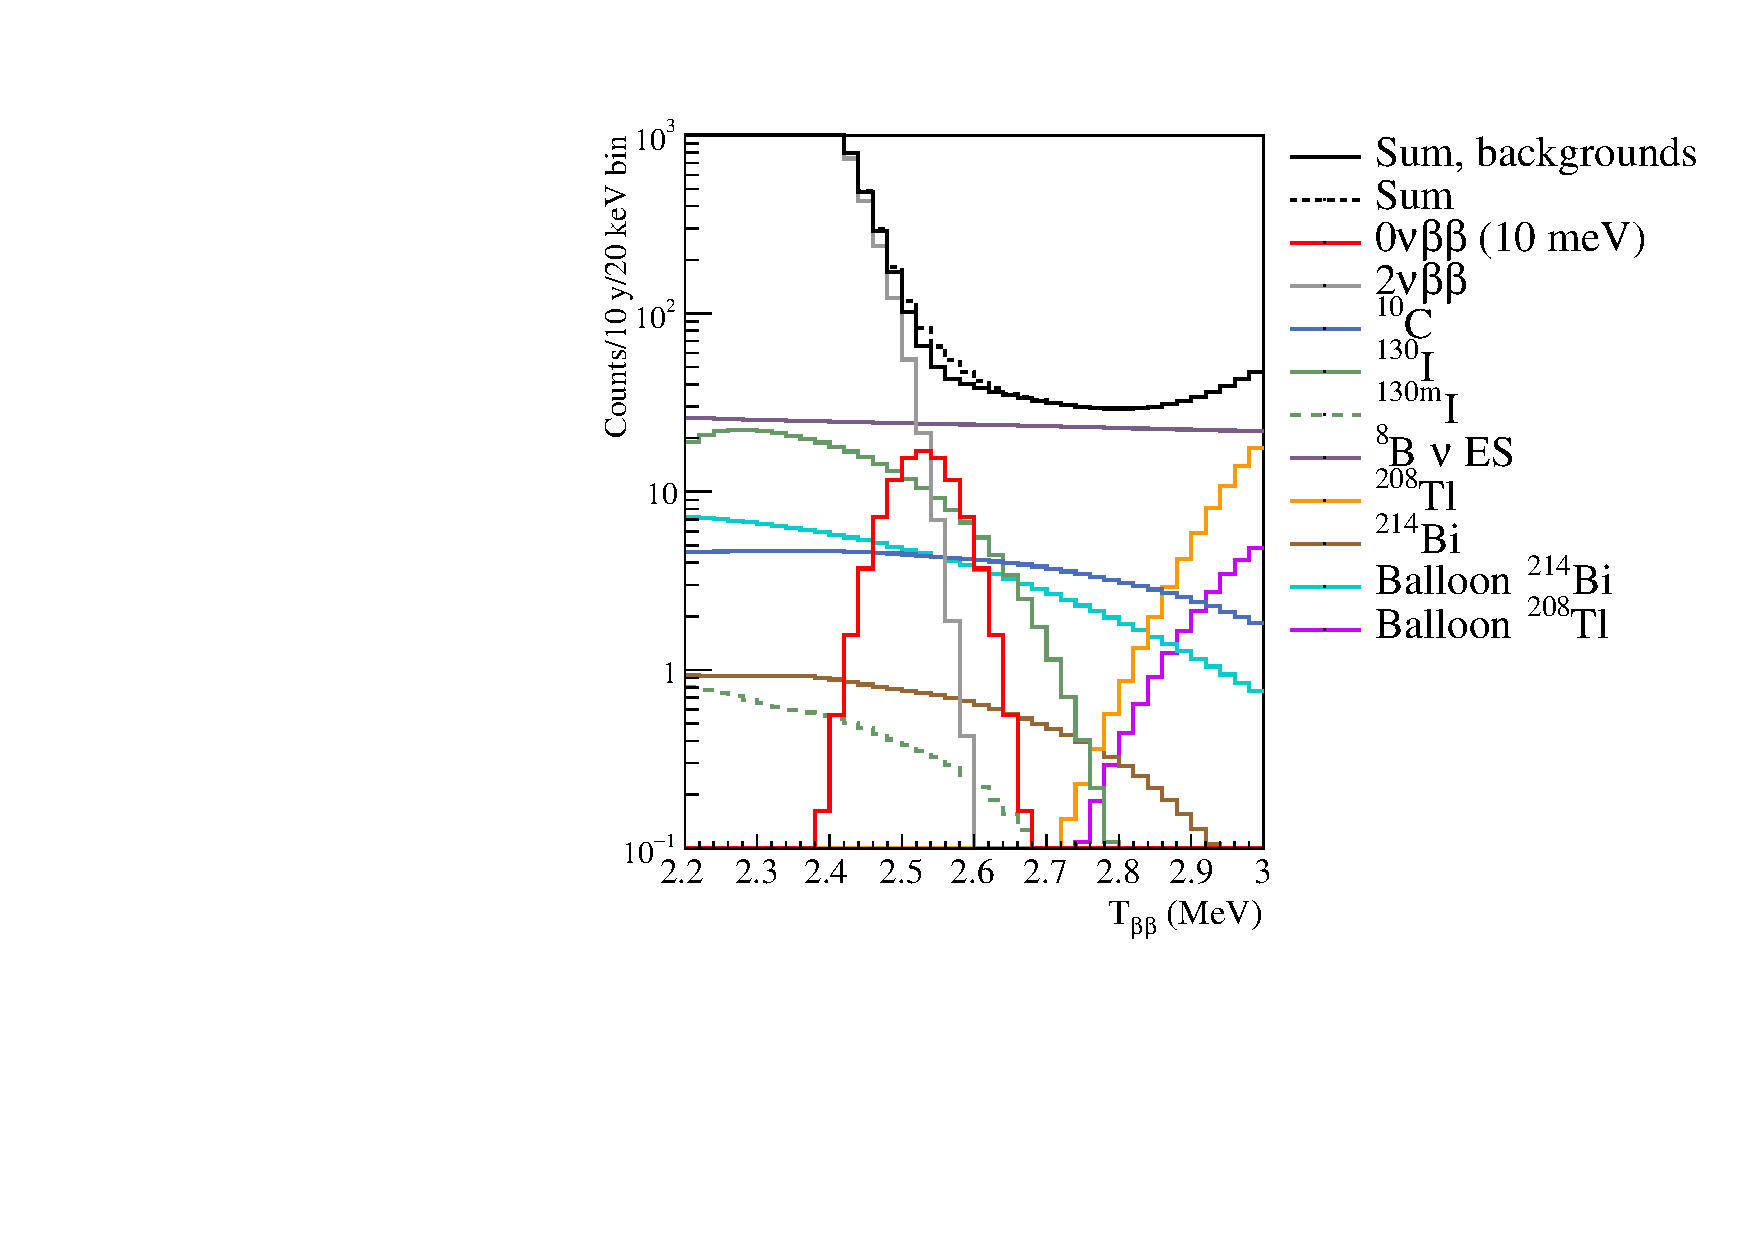
\includegraphics[width=\textwidth]{dbd/spectrum_plot_te.pdf}
 \caption{Te loading}
 \label{fig:spectrum-te}
\end{subfigure}
\begin{subfigure}[b]{0.49\textwidth}
 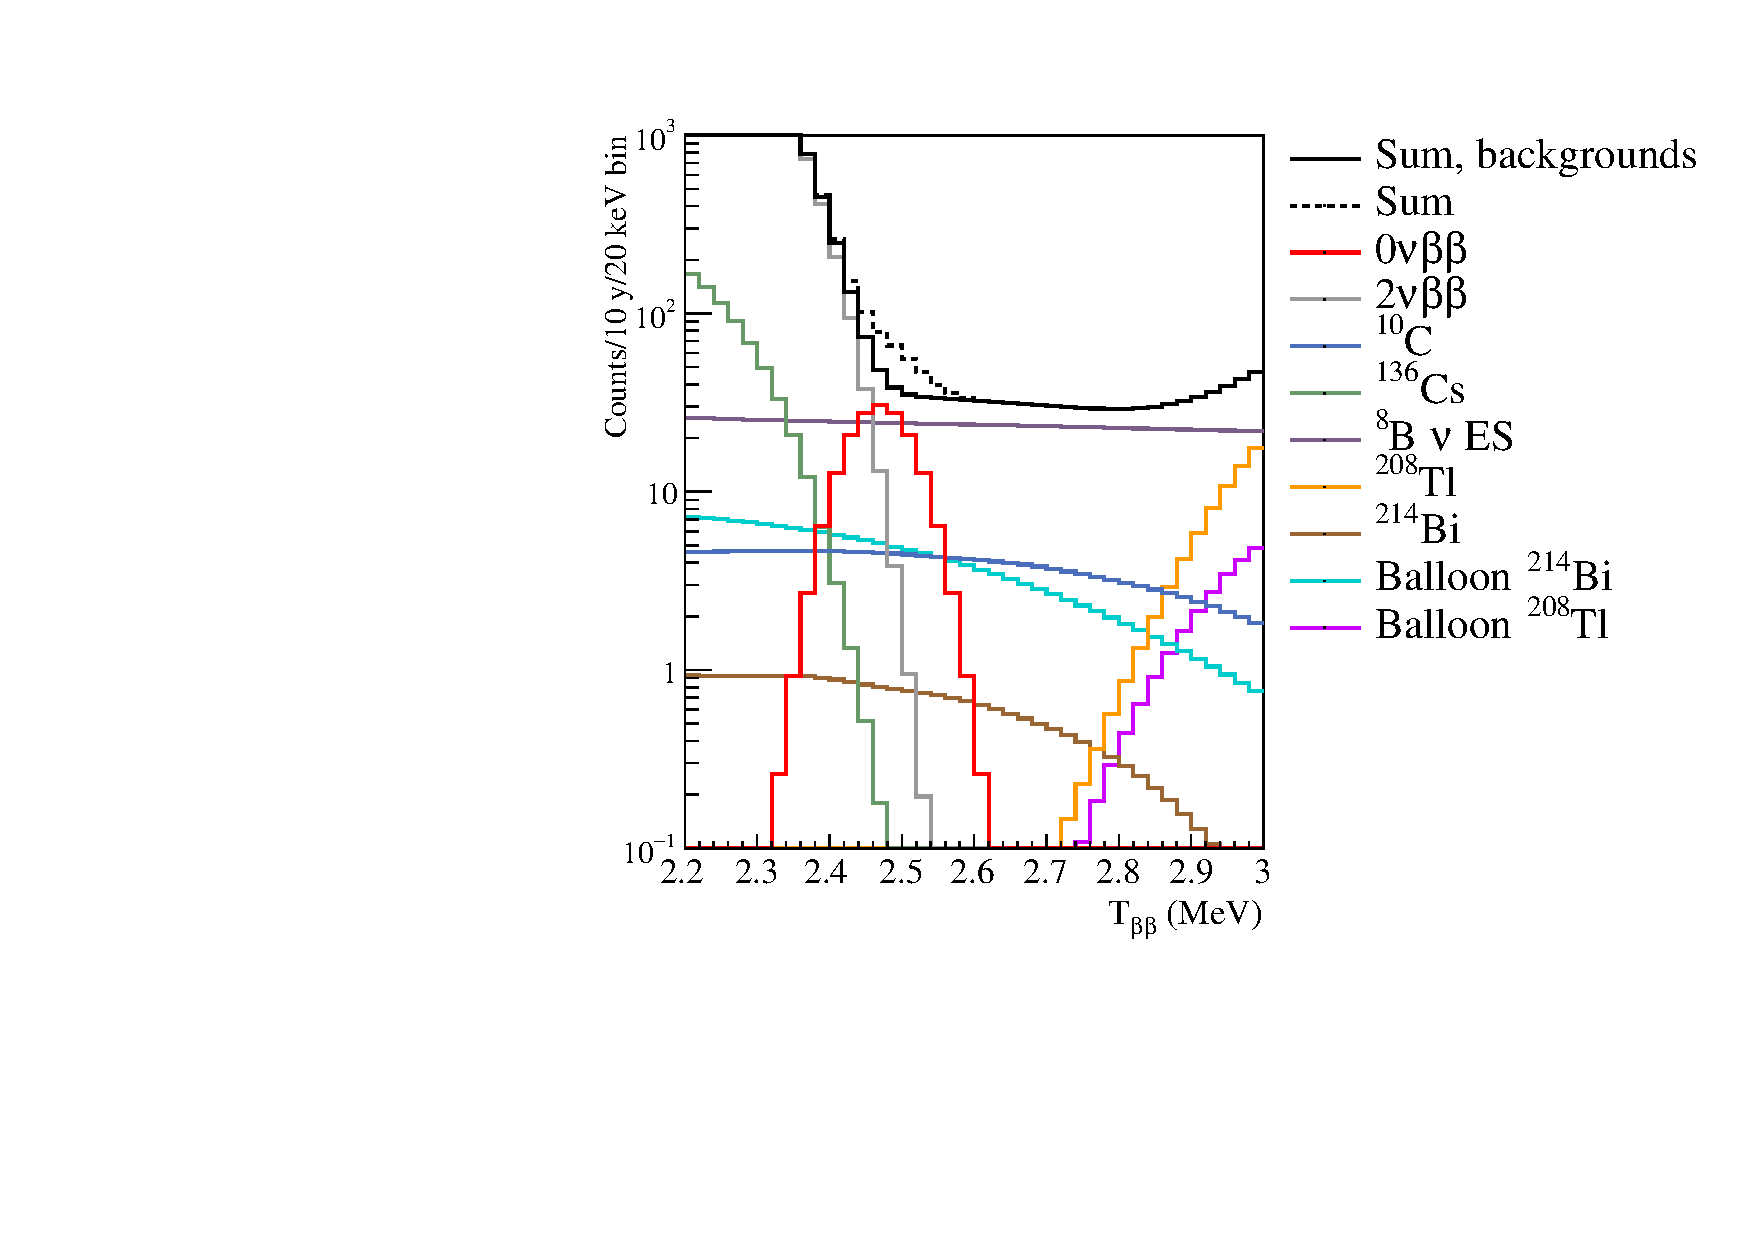
\includegraphics[width=\textwidth]{dbd/spectrum_plot_xe.pdf}
 \caption{Xe loading}
 \label{fig:spectrum-xe}
\end{subfigure}
\caption{Energy spectra near the NLDBD endpoint for events within the 7 m
fiducial volume.}
\label{fig:spectrum-plots}
\end{figure}

Following Equation \ref{eq:sens}, we obtain a sensitivity in terms of
$\hat{T}_{1/2}^{0\nu\beta\beta}$, and compute a corresponding limit on
the effective Majorana neutrino mass $m_{\beta\beta}$ assuming a light
neutrino exchange model with phase space factors from
Kotila and Iachello \cite{2012PhRvC..85c4316K} and using the IBM-2 matrix
element \cite{Barea:2013wb} for definiteness. The 90\% CL sensitivity
is:
\[
\mathrm{\bf Te:}~~
  T_{1/2}^{0\nu\beta\beta} > 9.7\times10^{27}~\mathrm{y},~
  m_{\beta\beta} < 6.7~\mathrm{meV}
\]
\[
\mathrm{\bf Xe:}~~
  T_{1/2}^{0\nu\beta\beta} > 2.6\times10^{28}~\mathrm{y},~
  m_{\beta\beta} < 4.9~\mathrm{meV}
\]

\noindent
%{\bf TODO:} Comment on prohibitive Xe costs?

\subparagraph{Energy Resolution}
The sensitivity is strongly dependent on the energy resolution, which in turn
depends on the total detected light yield, since this sets of the level to
which events in the steeply-falling $2\nu\beta\beta$ decay spectrum can
migrate into the NLDBD energy ROI. Figure \ref{fig:scale-ly} shows the
impact, holding other assumptions fixed.

\subparagraph{Solar Neutrinos}
It is possible in principle to discriminate solar neutrino interactions from
NLDBD signal, using Cherenkov light to determine the direction with respect
to the Sun and possibly separate one- and two-ring topologies, on a
statistical basis if not event-by-event. This is particularly important for
\textsc{Theia}, where solar neutrinos are expected to be the largest
background. Figure \ref{fig:scale-b8} shows the sensitivity scaling with solar
neutrino event rejection.

\subparagraph{U/Th Chain Backgrounds}
The level of internal and external U and Th chain background reduction also
depends on the power of timing and topology-based particle identification
methods. Figures \ref{fig:scale-ext} and \ref{fig:scale-bi214} show the
sensitivity as a function of the external background and $^{214}$Bi reduction
factors, respectively, with other parameters fixed.

\begin{figure}
\centering
\begin{subfigure}[b]{0.49\textwidth}
 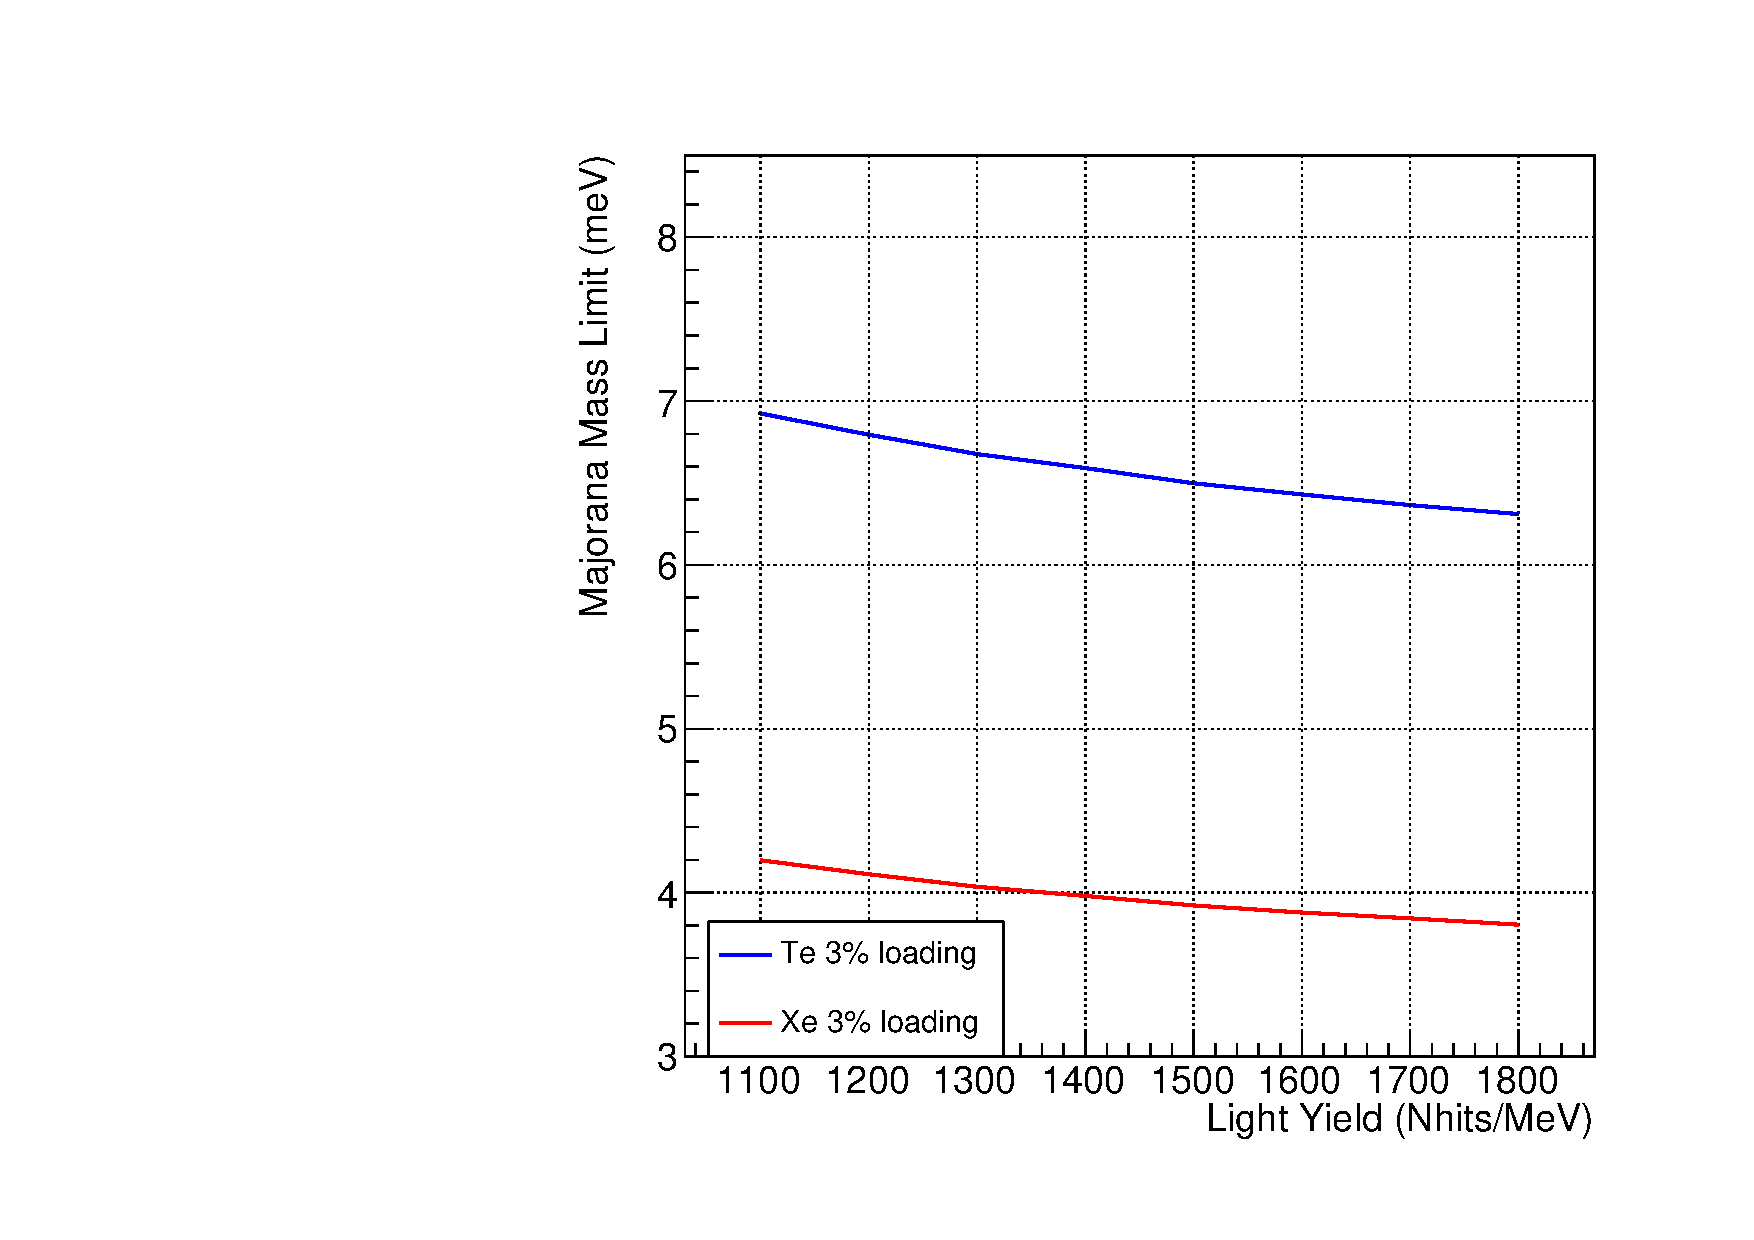
\includegraphics[width=\textwidth]{dbd/ly.pdf}
 \caption{Total detected light yield}
 \label{fig:scale-ly}
\end{subfigure}
\begin{subfigure}[b]{0.49\textwidth}
 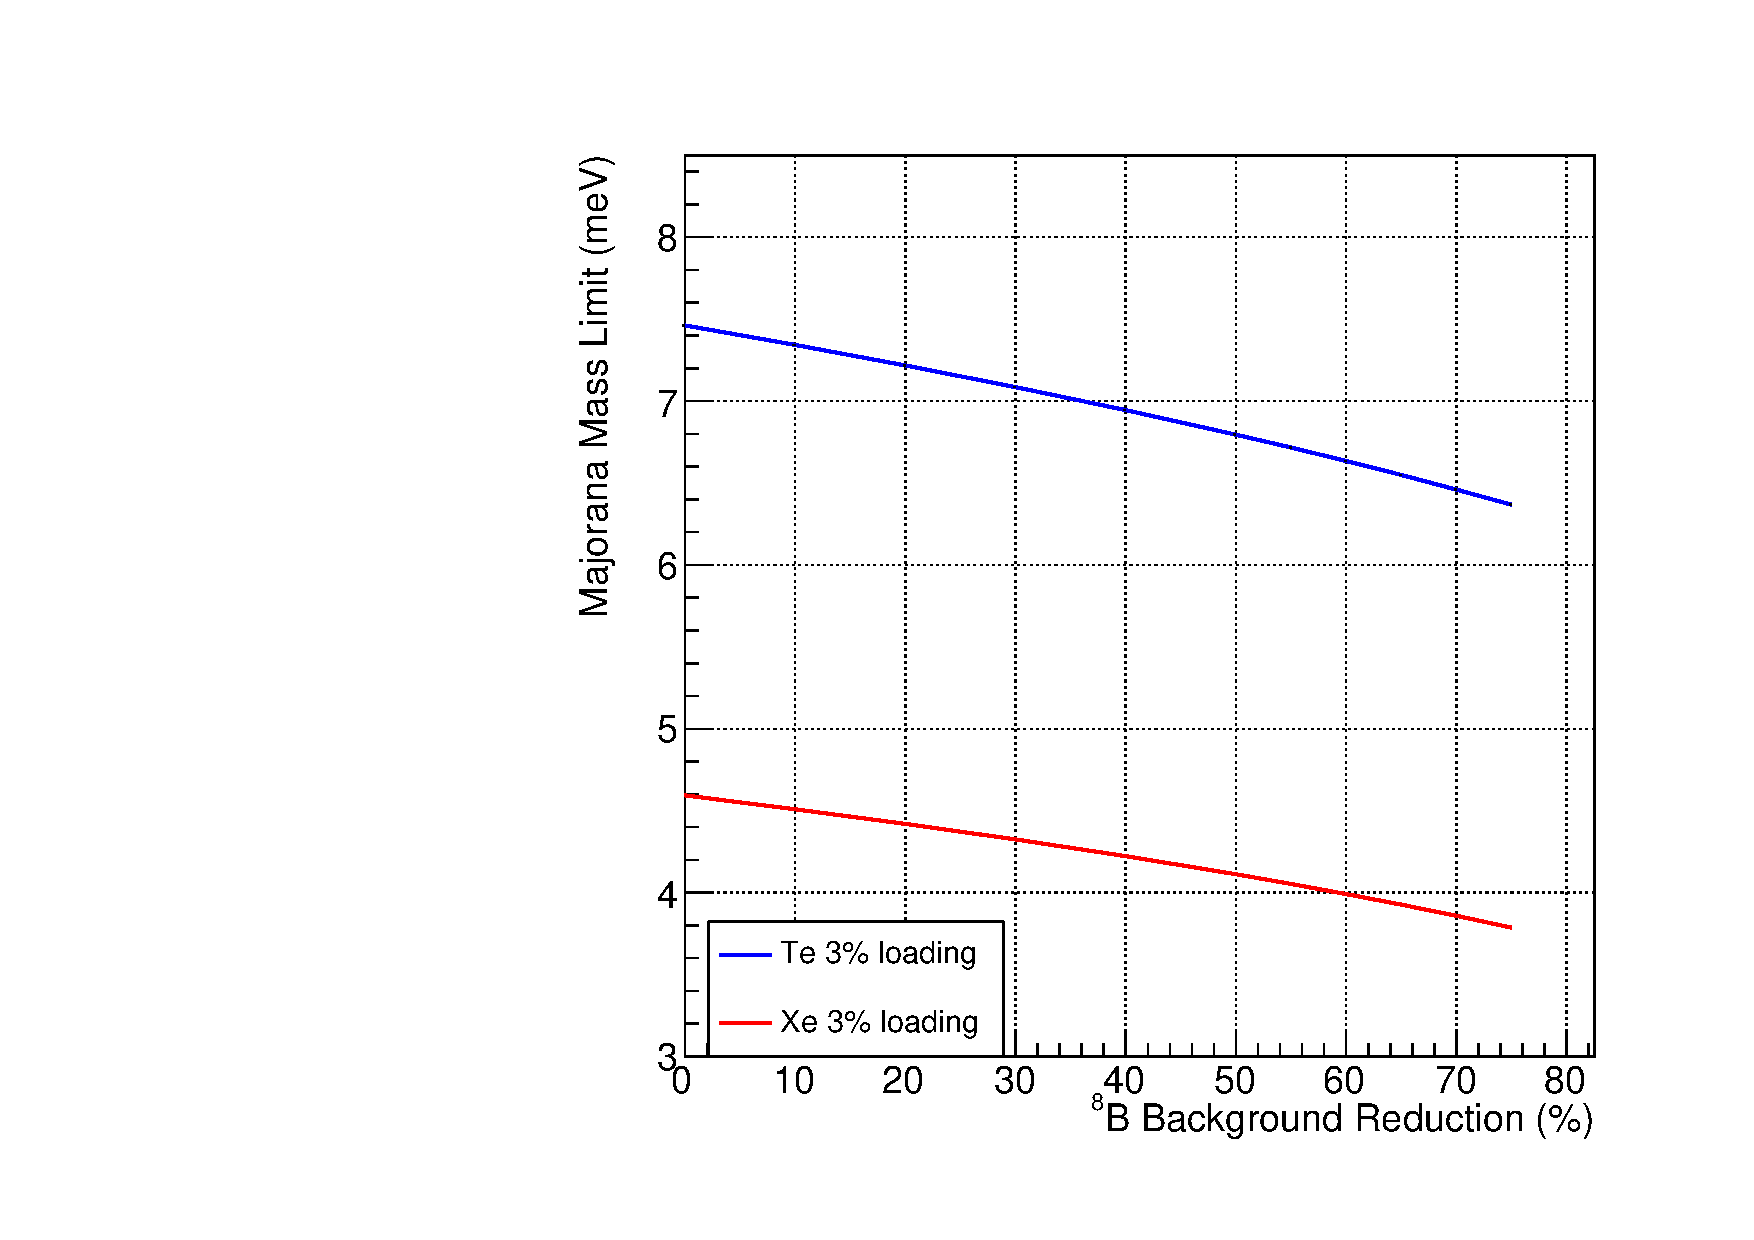
\includegraphics[width=\textwidth]{dbd/b8_reduction.pdf}
 \caption{Reduction factor for $^8$B solar neutrinos}
 \label{fig:scale-b8}
\end{subfigure}\\
\begin{subfigure}[b]{0.49\textwidth}
 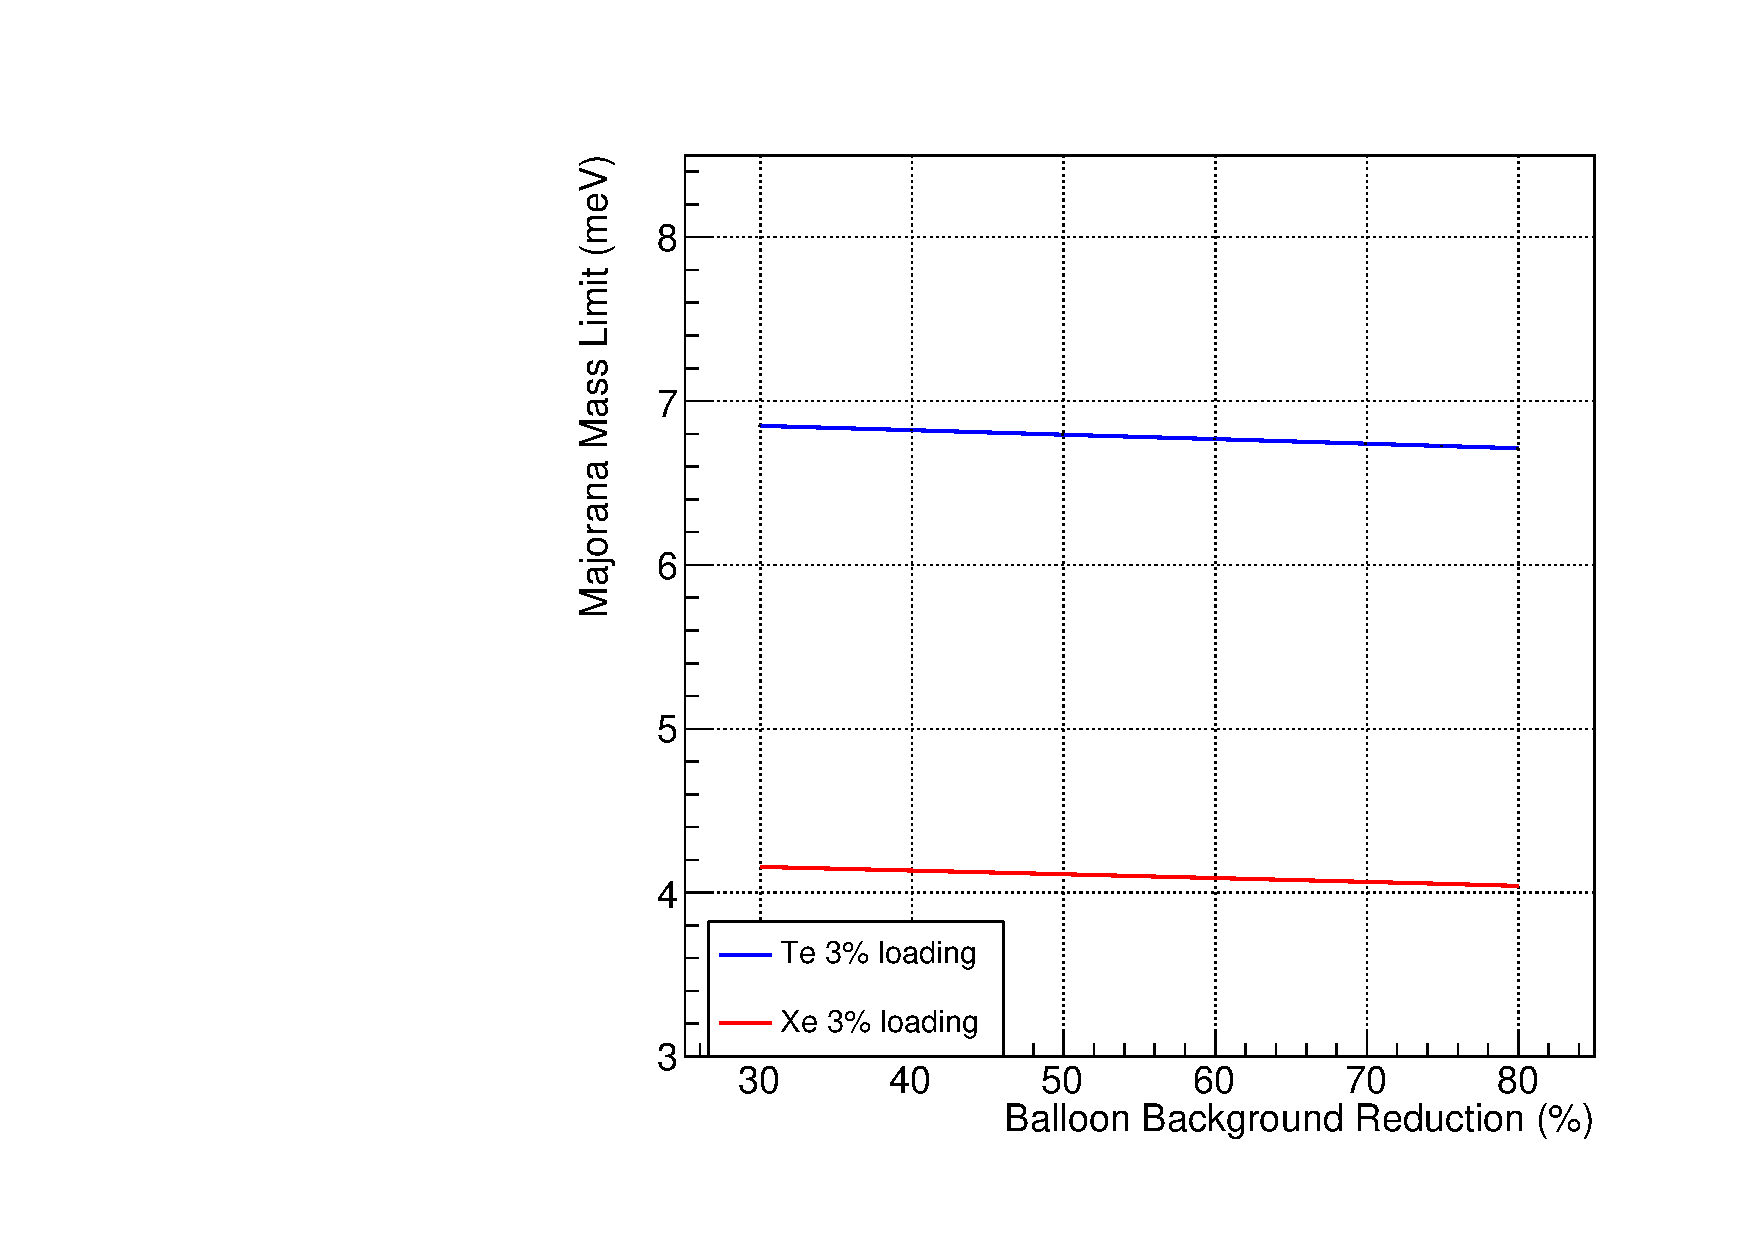
\includegraphics[width=\textwidth]{dbd/externals_reduction.pdf}
 \caption{Reduction factor for external backgrounds}
 \label{fig:scale-ext}
\end{subfigure}
\begin{subfigure}[b]{0.49\textwidth}
 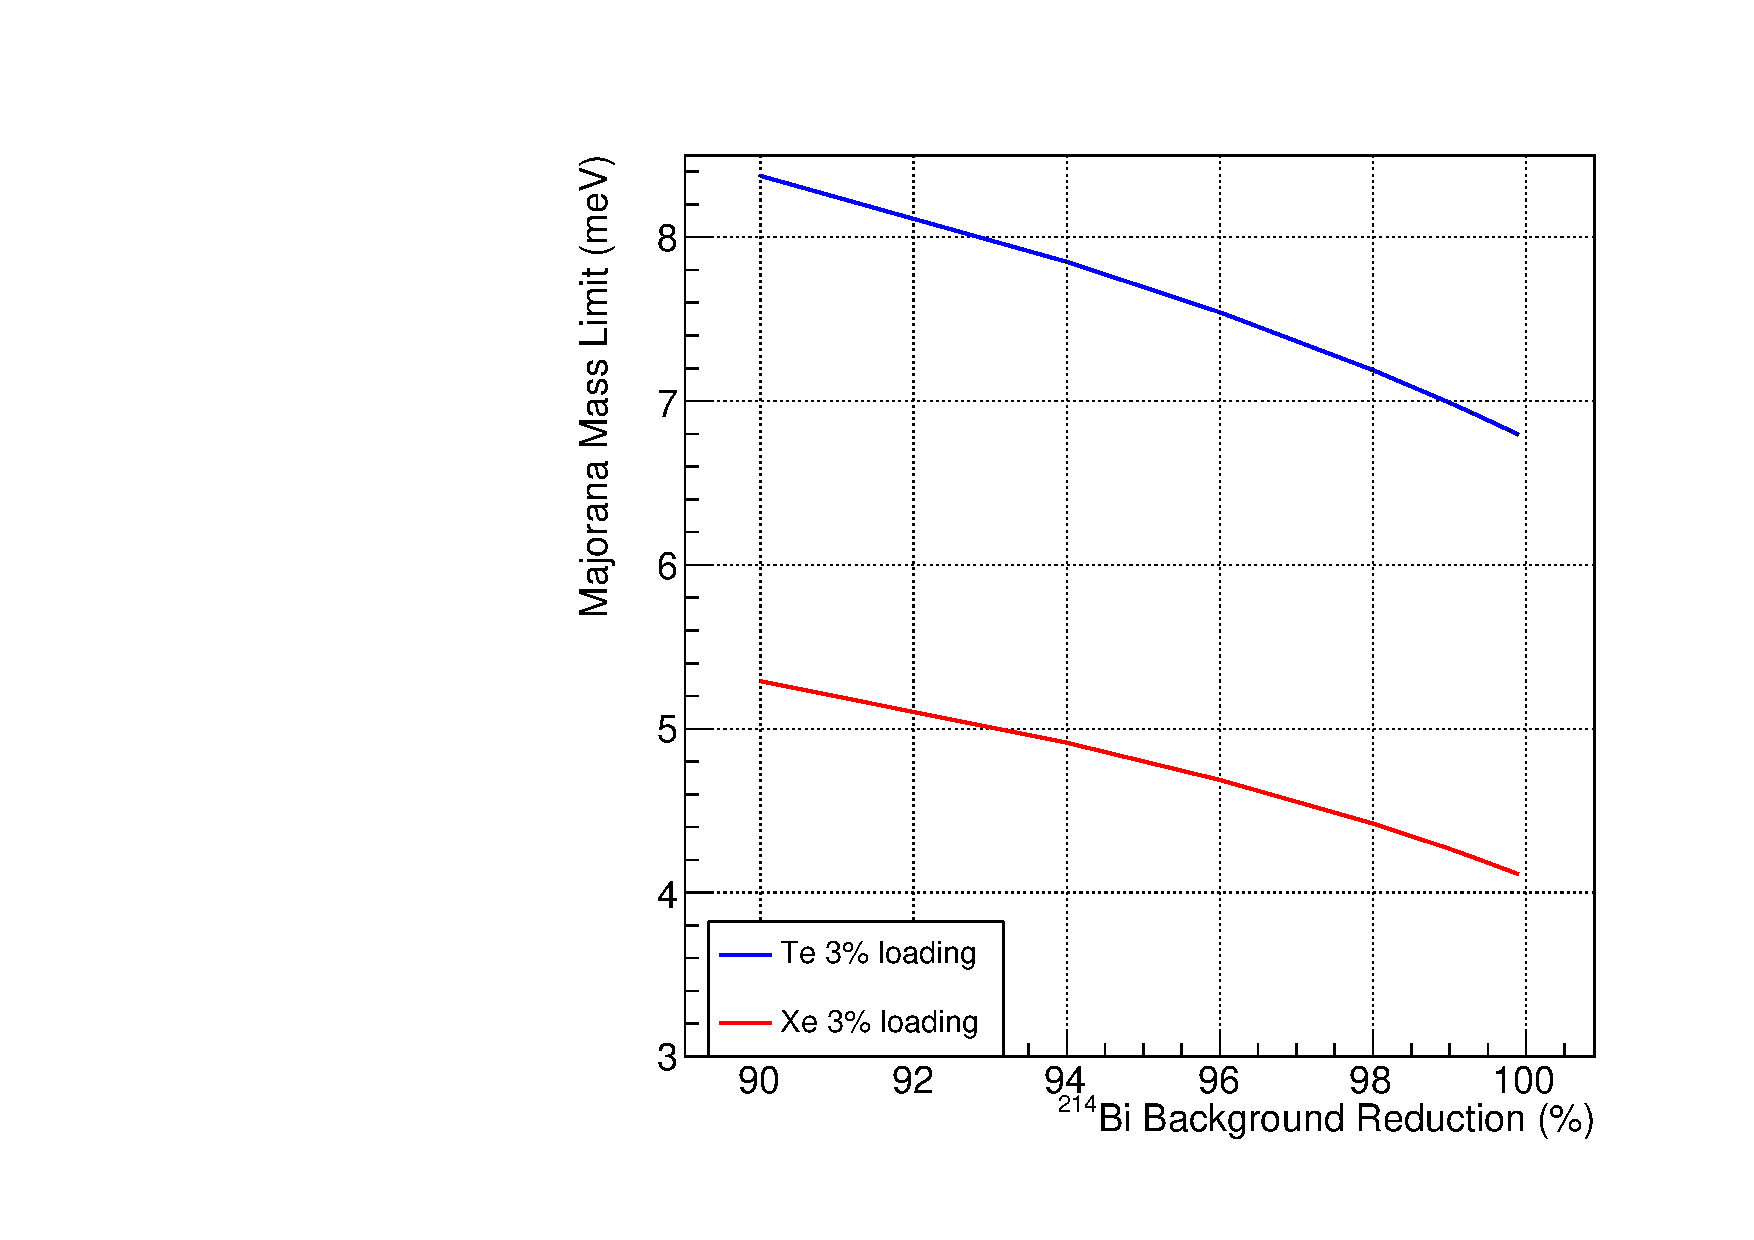
\includegraphics[width=\textwidth]{dbd/bi214_reduction.pdf}
 \caption{Reduction factor for $^{214}$Bi}
 \label{fig:scale-bi214}
\end{subfigure}
\caption{Mass sensitivity as a function of key experimental parameters.}
\label{fig:scaling-plots}
\end{figure}

\subsubsection{Conclusions}
In summary, the \textsc{Theia} experiment can perform a very sensitive search
for NLDBD, assuming a high level of Te or Xe loading and background levels
near those demonstrated by previous experiments. We have performed a
single-bin sensitivity analysis considering the dominant backgrounds for
an experiment located at the 4850 foot level of Homestake, accounting
for solar neutrino interactions, cosmogenic activation, and radioisotopic
contamination of detector materials. We have studied the behavior of these
backgrounds using a microphysical Monte Carlo simulation with a detector
model including scintillator and WbLS optics. We find that for aggressive
assumptions of radiopurity and background rejection, a \textsc{Theia} NLDBD
search is capable of reaching sensitivity within the non-degenerate normal
hierarchy parameter space.

%\section{Acknowledgements}
%
%\begin{thebibliography}{99}
%\bibitem{bxo16} N. Rossi, Neutrino 2016 Conference, London, 3---10 July 2016, \url{http://neutrino2016.iopconfs.org/IOP/media/uploaded/EVIOP/event_948/14.00__1_.pdf}
%\bibitem{mei09} D. M. Mei et al., Astropart. Phys. 31, 417–420 (2009).
%\bibitem{baudis15} L. Baudis et al., Eur. Phys. J. C 75, 485 (2015).
%\bibitem{zhang16} C. Zhang et al., Astropart. Phys. 84, 62--69 (2016).
%\bibitem{norm05} E. B. Norman et al., Nucl. Phys. B (Proc. Suppl.) 143, 508 (2005).
%\bibitem{bard97} D.W. Bardayan et al., Phys. Rev. C 55, 820 (1997).
%\bibitem{wang15} B.S. Wang et al., Phys. Rev. C 92, 024620 (2015).
%\bibitem{lozza15}  V. Lozza and J. Petzoldt, Astropart. Phys. 61, 62--71 (2015).
%\bibitem{snop16} S. Andringa et al., Advances in High Energy Physics 2016, 6194250 (2016).
%\bibitem{galb05} C. Galbiati, A. Pocar, D. Franco, A. Ianni, L. Cadonati, S. Schoenert, Phys.Rev. C 71 055805 (2005).
%\bibitem{gando16} Y Gando, Nuclear and Particle Physics Proceedings, vol. 273- 275, pp. 1842-1846 (2016).
%\bibitem{hagn00} T. Hagner et al., Astro. Phys. 14, 33--47, (2000).
%\bibitem{mei06} D. M. Mei and A. Hime, Phys. Rev. D 73, 053004 (2006).
%\bibitem{zbiri10} K. Zbiri, arxiv:0910.3714v3 [hep--ph] (2010).
%\bibitem{bxo2013} Borexino Collaboration, G. Bellini et al., JCAP08 49 (2013).
%\bibitem{SNO_3ph} SNO Collaboration, B. Aharmim et al., Physical Review C 88, 025501 (2013).
%\bibitem{Cuore017} C. Alduino et al., Eur. Phys. J. C 77 (2017).
%\bibitem{exo14}  J.B. Albert et al., Phys. Rev. C 89, 015502 (2014). 
%\bibitem{kam03} KamLAND Collaboration, K. Eguchi et al., Physical Review Letters 90, 021802, (2003).
%\bibitem{bxo09} Borexino Collaboration, C. Arpesella et al., Physical Review Letters 101,091302, (2008).
%\bibitem{gando13} A. Gando et al. Phys. Rev. Lett. 110, 062502 (2013).
%\bibitem{radiopurityorg} \url{https://www.radiopurity.org/rp/rp/_design/persephone/index.html?all}
%\bibitem{kamLAND_Zen} I. Shimizu, Frontiers of liquid Scintillator Technology (FroST16), March 18, 2016
%\url{https://indico.fnal.gov/getFile.py/access?contribId=45&sessionId=25&resId=0&materialId=slides&confId=10355}
%\bibitem{eijiri14} H. Ejiri and S. R. Elliott, Phys. Rev. C 89, 055501, (2014).
%\bibitem{eijiri17} H. Ejiri and S. R. Elliott, Phys. Rev. C 95, 055501 (2017).
%\bibitem{decay0} O.A.Ponkratenko, V.I.Tretyak, Yu.G.Zdesenko, Phys. At. Nucl. 63, 1282   (2000)  (nucl-ex/0104018)
%\bibitem{2012PhRvC..85c4316K} Kotila, J., \& Iachello, F. (2012). Phase-space factors for double-$\beta$ decay. Physical Review C - Nuclear Physics, 85(3), 034316. http://doi.org/10.1103/PhysRevC.85.034316
%\bibitem{Barea:2013wb} Barea, J., Kotila, J., \& Iachello, F. (2013). Nuclear matrix elements for double-$\beta$ decay. Physical Review C - Nuclear Physics, 87(1).
%\end{thebibliography}
%
%%\bibliographystyle{alpha}
%%\bibliography{sample}
%
%\end{document}

